\documentclass[10pt,a4paper]{article}
\usepackage{amssymb} %mathbb
\usepackage{amsmath} %align
\usepackage{graphicx} %jpg
\usepackage{tikz-cd}
\usepackage[top=1.0cm,bottom=1.3cm,left=1.0cm,right=1.0cm]{geometry}
\usepackage{array,bm}
\newcolumntype{L}{>{$}l<{$}}
\newcolumntype{C}{>{$}c<{$}}
\renewcommand{\arraystretch}{1.2}
\begin{document}

	\normalsize

		Whole mathematics $-$ without categories $-$ is context free. By Vinicius Claudino Ferraz.

		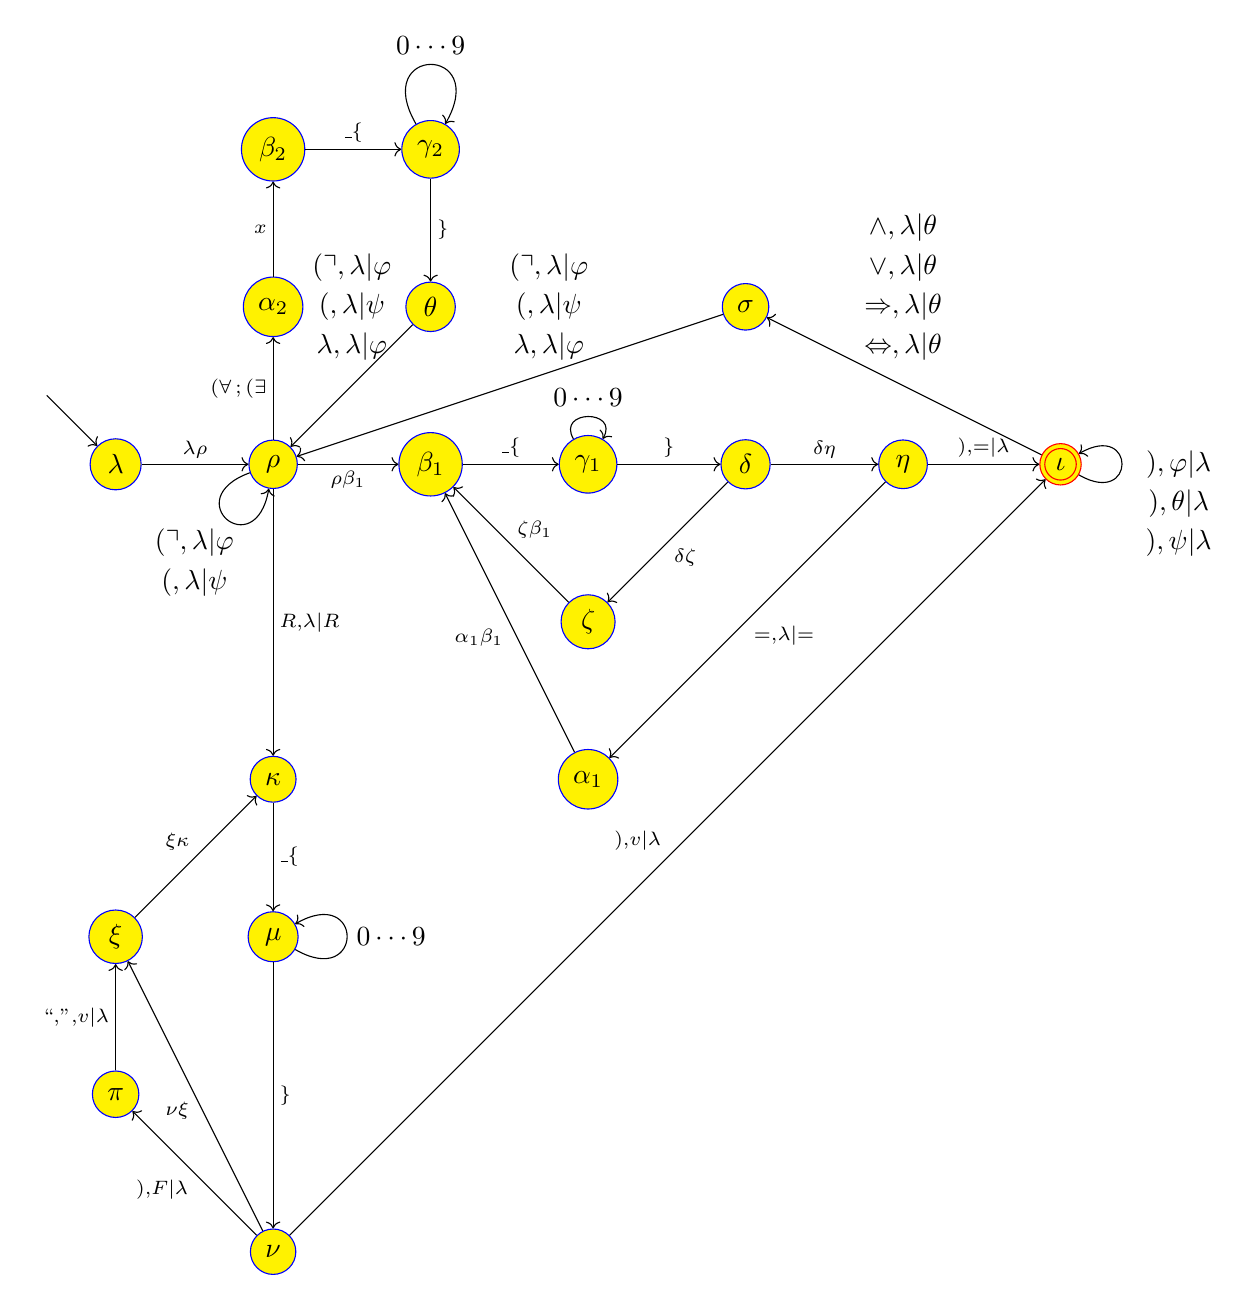
\begin{tikzpicture}
		\node (nada) at (0,1) { };
		\node[draw=blue, circle, fill=yellow] (lambda) at (1,0) {$\lambda$};
		\node[draw=blue, circle, fill=yellow] (rho) at (3,0) {$\rho$};
		\node (rholinha1) at (2,-1) {$(\urcorner, \lambda|\varphi$};
		\node (rholinha2) at (2,-1.5) {$(, \lambda|\psi$};
		\node[draw=blue, circle, fill=yellow] (alpha2) at (3,2) {$\alpha_2$};
		\node (alpha2linha1) at (4,2.5) {$(\urcorner, \lambda|\varphi$};
		\node (alpha2linha2) at (4,2) {$(, \lambda|\psi$};
		\node (alpha2linha3) at (4,1.5) {$\lambda, \lambda|\varphi$};
		\node (alpha2linha4) at (6.5,2.5) {$(\urcorner, \lambda|\varphi$};
		\node (alpha2linha5) at (6.5,2) {$(, \lambda|\psi$};
		\node (alpha2linha6) at (6.5,1.5) {$\lambda, \lambda|\varphi$};
		\node[draw=blue, circle, fill=yellow] (beta2) at (3,4) {$\beta_2$};
		\node[draw=blue, circle, fill=yellow] (gamma2) at (5,4) {$\gamma_2$};
		\draw[->] (gamma2) to [in=60,out=120, loop, "$0\cdots9$"] node { } (gamma2);
		\draw[->] (rho) to [in=260,out=200, loop, " "] node { } (rho);
		\node[draw=blue, circle, fill=yellow] (theta) at (5,2) {$\theta$};
		\node[draw=blue, circle, fill=yellow] (beta1) at (5,0) {$\beta_1$};
		\node[draw=blue, circle, fill=yellow] (gamma1) at (7,0) {$\gamma_1$};
		\draw[->] (gamma1) to [in=60,out=120, loop, looseness=3, "$0\cdots9$"] node { } (gamma1);
		\node[draw=blue, circle, fill=yellow] (zeta) at (7,-2) {$\zeta$};
		\node[draw=blue, circle, fill=yellow] (alpha1) at (7,-4) {$\alpha_1$};
		\node[draw=blue, circle, fill=yellow] (kappa) at (3,-4) {$\kappa$};
		\node[draw=blue, circle, fill=yellow] (mu) at (3,-6) {$\mu$};
		\draw[->] (mu) to [in=30,out=330, loop, " "] node { } (mu);
		\node (mulinha) at (4.5,-6) {$0\cdots9$};
		\node[draw=blue, circle, fill=yellow] (nu) at (3,-10) {$\nu$};
		\node[draw=blue, circle, fill=yellow] (pi) at (1,-8) {$\pi$};
		\node[draw=blue, circle, fill=yellow] (xi) at (1,-6) {$\xi$};
		\node[draw=blue, circle, fill=yellow] (delta) at (9,0) {$\delta$};
		\node[draw=blue, circle, fill=yellow] (sigma) at (9,2) {$\sigma$};
		\node (sigmalinha1) at (11, 3) {$\wedge, \lambda|\theta$};
		\node (sigmalinha2) at (11,2.5) {$\vee, \lambda|\theta$};
		\node (sigmalinha3) at (11,2) {$\Rightarrow, \lambda|\theta$};
		\node (sigmalinha4) at (11,1.5) {$\Leftrightarrow, \lambda|\theta$};
		\node[draw=blue, circle, fill=yellow] (eta) at (11,0) {$\eta$};
		\node[draw=red, circle, fill=yellow] (iota) at (13,0) {$\iota$};
		\node (iotalinha1) at (14.5, 0) {$), \varphi|\lambda$};
		\node (iotalinha2) at (14.5, -0.5) {$), \theta|\lambda$};
		\node (iotalinha3) at (14.5, -1) {$), \psi|\lambda$};
		\draw[red] (13,0) circle (0.2);
		\draw[->] (iota) to [in=30,out=330, loop, " "] node { } (iota);
		\path[commutative diagrams/.cd, every arrow, every label]
		(nada) edge node { } (lambda)
		(lambda) edge node {$\lambda\rho$} (rho)
		(rho) edge node[swap] {$\rho\beta_1$} (beta1) edge node {$R, \lambda|R$} (kappa) edge node {$(\forall\,;\,(\exists$} (alpha2)
		(alpha2) edge node {$x$} (beta2)
		(beta2) edge node {$\_\{$} (gamma2)
		(gamma2) edge node {$\}$} (theta)
		(theta) edge node { } (rho)
		(iota) edge node { } (sigma)
		(sigma) edge node { } (rho)
		(kappa) edge node {$\_\{$} (mu)
		(mu) edge node {$\}$} (nu)
		(nu) edge node {$), v|\lambda$} (iota) edge node {$), F|\lambda$} (pi) edge node {$\nu\xi$} (xi)
		(pi) edge node {$``,", v|\lambda$} (xi)
		(xi) edge node {$\xi\kappa$} (kappa)
		(beta1) edge node {$\_\{$} (gamma1)
		(gamma1) edge node {$\}$} (delta)
		(delta) edge node {$\delta\eta$} (eta) edge node {$\delta\zeta$} (zeta)
		(eta) edge node {$), =|\lambda$} (iota) edge node {$=, \lambda|=$} (alpha1)
		(zeta) edge node[swap] {$\zeta\beta_1$} (beta1)
		(alpha1) edge node {$\alpha_1\beta_1$} (beta1);
		\end{tikzpicture}

		\vspace{3mm}

		\begin{tabular}{|C|C|L}
		  \cline{1-2}
		  \lambda\rho & (\urcorner, \lambda|\varphi & \textbf{not} \\
		   & (, \lambda|\psi  \\
		   & \lambda  \\
		  \cline{1-2}
		  \rho\beta_1 & (x, \lambda|x & \textbf{variable} \\
		   & (c, \lambda|c & \textbf{constant}  \\
		   & (f, \lambda|f & \textbf{function} \\
		  \cline{1-2}
		  \delta\eta & ), v|\lambda \\
		   & \lambda, c|\lambda \\
		   & \lambda, x|\lambda \\
		  \cline{1-2}
		  \delta\zeta & (, f|\lambda \\
		  & ``,", v|\lambda & \textbf{comma between parameters} \\
		  \cline{1-2}
		  \zeta\beta_1 & x, \lambda|v \\
		  & c, \lambda|v \\
		  \cline{1-2}
		  \alpha_1\beta_1 & x, \lambda|x \\
		   & c, \lambda|c  \\
		   & f, \lambda|f \\
		  \cline{1-2}
		  \nu\xi & (, R|\lambda \\
		  & ``,", v|\lambda \\
		  & (, f|F \\
		  \cline{1-2}
		  \xi\kappa & x, \lambda|v \\
		   & c, \lambda|v \\
		    & f, \lambda|vf \\
		  \cline{1-2}
		\end{tabular}

		\vspace{120mm}

		I'm going to post some figures for dummies.

		\begin{center}
		\includegraphics[scale=.5]{21}
		\end{center}

		\begin{center}
		\includegraphics[scale=.5]{31}
		\end{center}

		\begin{center}
		\includegraphics[scale=.5]{32}
		\end{center}

		For instance:

		\begin{center}
		\includegraphics[scale=1]{exemplos}
		\end{center}

\end{document}
